\section{Introduction}\label{intro}

\subsection{Online Social Networks}
 
In recent years, online social networks (OSNs) have been utilised as
means to express ideas and opinions, spread information about events,
or even stimulate and propagate calls for civic engagement and
societal action. Social networking sites such as Twitter, Facebook,
LinkedIn and YouTube have also empowered individuals to promote their
viewpoints and interests -- professional or otherwise -- to a broad
and diverse global audience. The engagement of certain demographics
with social networks offers the opportunity for researchers interested
in observing and interpreting society to apply established theory and
methods to an emerging digital culture.

To satisfy the demand for various types of communities, interactions
and engagement, there are now vast numbers of social media sites and
platforms\footnote{This list is by no means exhaustive:
\url{http://en.wikipedia.org/wiki/List of social networking
websites}}, along with a number of attempted categorisations. By 2018,
there will be an estimated 2.5 billion active social network users (up
from 1.9 billion in 2014); they are producing massive amounts of data
(volume) on a real-time basis (velocity) with implicit sociological
attributes such as beliefs, opinions, sentiments, behaviours,
structures and influences (variety)~\cite{burnap-et-al:2015}. These
data exhibit the key traits of what is now referred to as big data:
volume, velocity and variety~\cite{postsm:2014}. In this age of big
data and an increasingly interconnected digital society, there is a
new challenge -- the application of robust and scalable methods and
tools that can be applied to digitised social behaviour generated via
social networks so as to be able to efficiently analyse big social
data to provide insight into real-world events and
actions~\cite{lazer-et-al:2009,burnap-et-al:2015}.

Recent
work~\cite{blamey-et-al-2012,schwartz-et-al:2013,blamey-et-al-2013,oatley+crick:2014,mostafa-et-al-ai2016}
has analysed what people say on social media to identify distinctive
words, phrases, and topics as functions of known attributes of people
such as gender, age, location, or psychological characteristics. This
can thus be collated and aggregated, inferring gender, age, location
and sentiments, from social media data. Potential negative
implications of these approaches include the fact that they can be
easily applied to large numbers of people or groups in society without
obtaining their explicit consent or even being aware it is being
done. Data-driven commercial companies, governmental entities, or
even one's followers or friends are able to use software to infer
personality and other attributes -- such as sexual orientation or
political affiliations -- that an individual may have decided not to
share~\cite{lambiotte+kosinski:2014,postsm:2014}.

There are various projects that have used Twitter corpora and related
datasets to make predictions about
elections~\cite{tumasjan-et-al:2010}, stock
markets~\cite{zhang-et-al:2011}, and crimes and
policing~\cite{gerber:2014,oatley+crick:2015}. Twitter played an
important role during what was then known as the ``Arab Spring'',
which has been extensively examined in the social network analysis
domain~\cite{lotan-et-al:2011,howard-et-al:2011,comunello+anzera:2012,wolfsfeld-et-al:2013,bruns-et-al:2013}.
While the use of Twitter data has been demonstrated to provide insight
-- and sociologically relevant demographics~\cite{sloan-et-al:2013} --
into major social and physical events such as
riots~\cite{procter-et-al:2013} and terror
attacks~\cite{burnap-et-al:2014}, often all is not what it may seem;
for instance, many tweets may not a crowd
make~\cite{liang-et-al:2013}.

\subsection{Languages and Communities}

Despite the widespread engagement with Twitter globally, little
research has investigated the differences amongst users of various
languages; there is a tendency to assume that the behaviours of
English users generalise to other language
users~\cite{hong-et-al:2011}. Language has featured as a facet of
research on the geographies of Twitter
networks~\cite{takhteyev-et-al:2012}, especially whether offline
geography still matter in online social
networks~\cite{kulshrestha-et-al:2012}. Linguistic-inspired studies
have been done on hashtags~\cite{cunha-et-al:2011}, as well as the
volume and proportional of tweets in English and Arabic, as part of an
analysis of the Arab Spring~\cite{bruns-et-al:2013}. Nevertheless,
language is clearly a vital component of affiliation and discourse on
the web~\cite{zappavigna+martin:2012}, with the creation and curation
of emerging multilingual networks and communities, representing
well-established creative and cultural norms, including for minority
languages such as Welsh~\cite{gj+uj:2013}, as well as investigations
into the economics of linguistic
diversity~\cite{ginsburgh+weber:2011}.

\subsection{Social Network Analysis}

In the social network analysis (SNA) domain, centrality measures
provide the ability to assess network graphs that are constructed from
collected data (for example, tweets). Selection of these centrality
measures is dependent on the goal of the analysis; for example, the
degree of node helps to identify nodes with high number of connections
within the
network~\cite{borgatti+everett:2000,rombach-et-al:2014,liu-et-al:2014}.
In a representation of a real world network, this metric may help to
identify highly connected persons, such as political leaders, sports
stars or celebrities, who are potential ``information
spreaders''~\cite{cha-et-al:2012,borge-holthoefer-et-al:2012,zhang-et-al:2016}.
Centrality measures such as degrees, betweenness, clustering
coefficient, modularity and cliques have been used in many projects to
measure influence or detect the emergence of new
communities~\cite{willis-et-al:2015,oatley+crick:2015}.

Clustering users in communities has been an important analytic factor
in social networking analysis; numerous work has focused on clustering
users based on their locations. However, for the sake of anonymity,
many users tend not to disclose information about their identity, such
as locations~\cite{kang-et-al:2013}. It has also been reported in the
literature that geotagged tweets are generally low in
number~\cite{morstatter-et-al:2013,tan-et-al:2013,kumar-et-al:2014},
the exponential growth in social media over the past decade has been
joined by the rise of location as a central organising
theme~\cite{liang-et-al:2013} of how users engage with online
information services and, more importantly, with each
other~\cite{cheng-et-al:2010,caverlee-et-al:2013}.

\subsection{Users and Location}

It is important to understand how geotagging works in Twitter. The
`place' entity included in a Twitter status does not necessarily
indicate precisely where the actual posting was made, as stated in the
Twitter API
documentation\footnote{\url{https://dev.twitter.com/overview/api/places}}:

\begin{quotation} ``{\emph{Tweets associated with places are not
necessarily issued from that location but could also potentially be
about that location.}}
\end{quotation}

For the sake of anonymity many users tend not to disclose information
about their identity, particularly locations; this has also been
supported by the literature that geotagged tweets are generally low in
number~\cite{kang-et-al:2013}. An alternative location-based option to
consider is based on profile location, but this may not serve the need
for location clustering for a multitude of reasons, especially with a
significant proportion of Twitter users not setting their profile
location~\cite{graham-et-al:2014}.

\subsection{Language Communities}\label{langcomm}

Analysis of language communities begins with two basic techniques. The
first is to classify statuses based on their languages. The status
language is extracted from the `{\emph{lang}}' entity inside status
objects. Language used in posting defines which community the status
was meant for; a tweet written in Turkish, for example, is meant for
the Turkish-speaking community. Output from this will be referred to
as `posting communities'. The second analysis is to classify users
into different communities based on their profile languages,
regardless of the posting language they used. Output from this
technique will be referred to as `profile communities'. As we will see
in the following two case studies, a posting community does not
necessarily indicate the profile community for a user. Therefore, the
second step is to examine the relationship between profile and posting
communities. We will also explore relationships amongst profile
communities, in term of action-reaction. We will investigate the
intra- and inter-profile communities interactions by constructing
network graphs and generate a visual representation.

\subsection{Overview of Paper}

The techniques we introduce in this paper through two real-world case
studies are based on language settings in users' profiles and those
for statuses\footnote{The term `status' is a generic term used to
refer to any Twitter post (tweet, retweet, reply, or quote).}. The
remainder of this paper is organised as follows:
Sections~\ref{baltimorecasestudy} and~\ref{eurovisioncasestudy}
presents the 2015 Baltimore protests and 2016 Eurovision Song Context
case studies, along with an analysis of the key data and
results. Section~\ref{conclusions} concludes the paper with a wider
discussion and a summary of the potential application of our approach.


\section{Case Study: 2015 Baltimore Protests}\label{baltimorecasestudy}

Following the peaceful funeral of Freddie Gray that took place on the
morning of Monday 27 April 2015 in Baltimore, Maryland, USA, a protest
hit the city. According to the timeline published on the CNN website
``{\emph{The city exploded on Monday after the funeral of Freddie
Gray, a 25-year-old black man who mysteriously died on April 19, a
week after Baltimore Police arrested
him.}}''~\cite{baltimorewiki:2015}. The nature of the Baltimore protests
is a good representation of a planned event in which a sudden
escalation of violence hits a geographical area. The event manifested
itself on Twitter as {\texttt{\#BaltimoreRiots}}, and resulted in more
than 1,250,000 status updates.

Figure~\ref{fig:overallbaltimoreactivity} and Figure~\ref{fig:mainevents}
present how the event manifested itself on Twitter once a ``purge'' was
scheduled. We can see that what was happening on the ground was
quickly reflected on the activity in Twitter, as
Figure~\ref{fig:mainevents} indicates. More detailed analysis reveals
that within one hour the topic started to go ``viral''; more
precisely, at approximately 15:00 at which the ``purge'' was
scheduled. The topic jumped from roughly 1,200 to 8,000 tweets per
hour. Then, it peaked with 98,000 between 22:00 and 23:00.

\begin{figure}[htb]
\centering
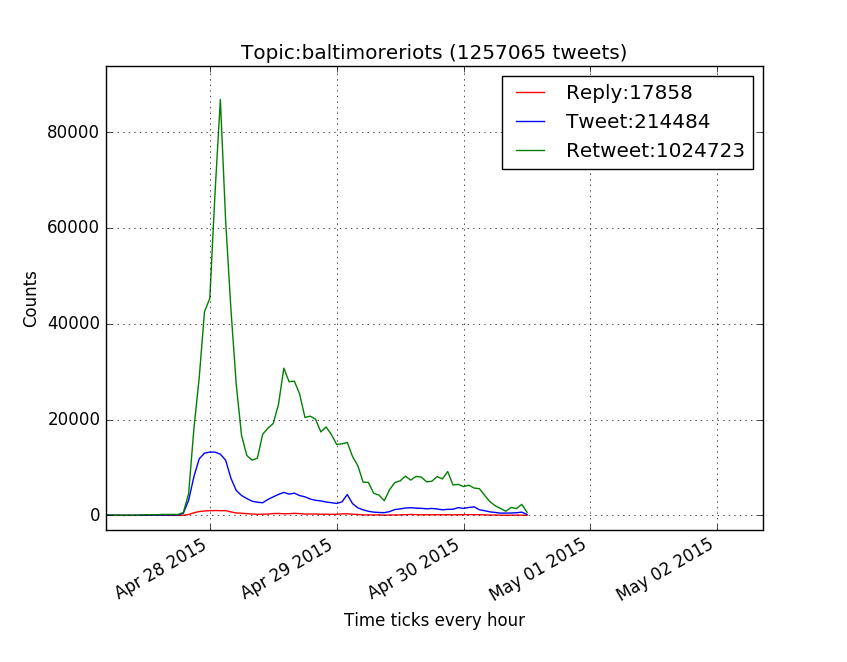
\includegraphics[width=\columnwidth]{images/overallbaltimoreactivity.png}
\caption{Overall activity for {\texttt{\#BaltimoreRiots}}.}
\label{fig:overallbaltimoreactivity}
\end{figure}

\begin{figure}[htb]
\centering
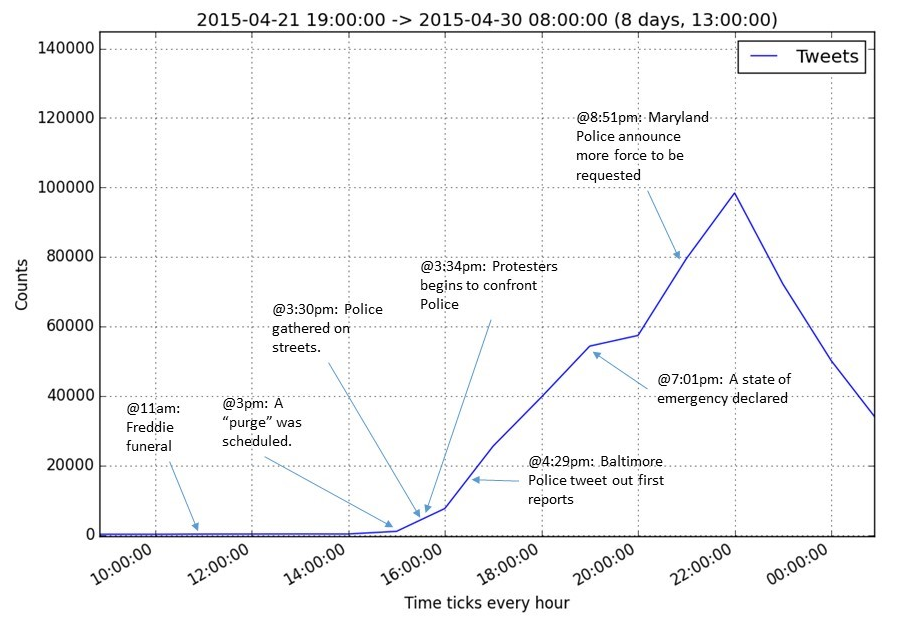
\includegraphics[width=\columnwidth]{images/mainevents.png}
\caption{Main events during the lifetime of {\texttt{\#BaltimoreRiots}}.}
\label{fig:mainevents}
\end{figure}

\subsection{Locations}\label{baltimorelocations}

As mentioned in Section~\ref{intro}, for the sake of anonymity many
users tend not to disclose information about their identity,
particularly locations; this has also been supported by the literature
that geotagged tweets are generally low in
number~\cite{kang-et-al:2013}. We took the step to verify this claim
in our datasets; in the best cases, the ratio of geotagged tweets did
not exceed 2\%. In the case of the {\texttt{\#BaltimoreRiots}}
dataset, only ~1\% of collected statuses were associated with
places. Moreover, out of this geotagged subset, only 4\% were
associated with the city where the event took place (Baltimore).

An alternative location-based option to consider is based on profile
location, but it still does not serve the need for location clustering
for a multitude of reasons. Firstly, we found that less than 45\% of
users have set their profile location, which is in line with other
studies~\cite{graham-et-al:2014}. Secondly, although Twitter suggests
certain presets for setting profile location, users are given the
option to enter any text they wish; this results in a considerable
amount of noise.

\subsection{Posting Communities}

In the {\texttt{\#BaltimoreRiots}} case, for original posts, there were 39 posting
languages, including und. As we can see in Figure~\ref{fig:baltimore_langfreq}, English was the
dominating language by far. Interestingly, results also show that
language of more than ~7\% statuses could not be
identified. When investigated, those statuses mostly do not contain
text other than hashtags, pictures or URLs. Although, this is not a
big portion, it came second after English. Although this category
shows an interesting case in which qualitative content analysis would
be involved, it is beyond this study and will not be covered here.

\begin{figure}[htb]
\centering
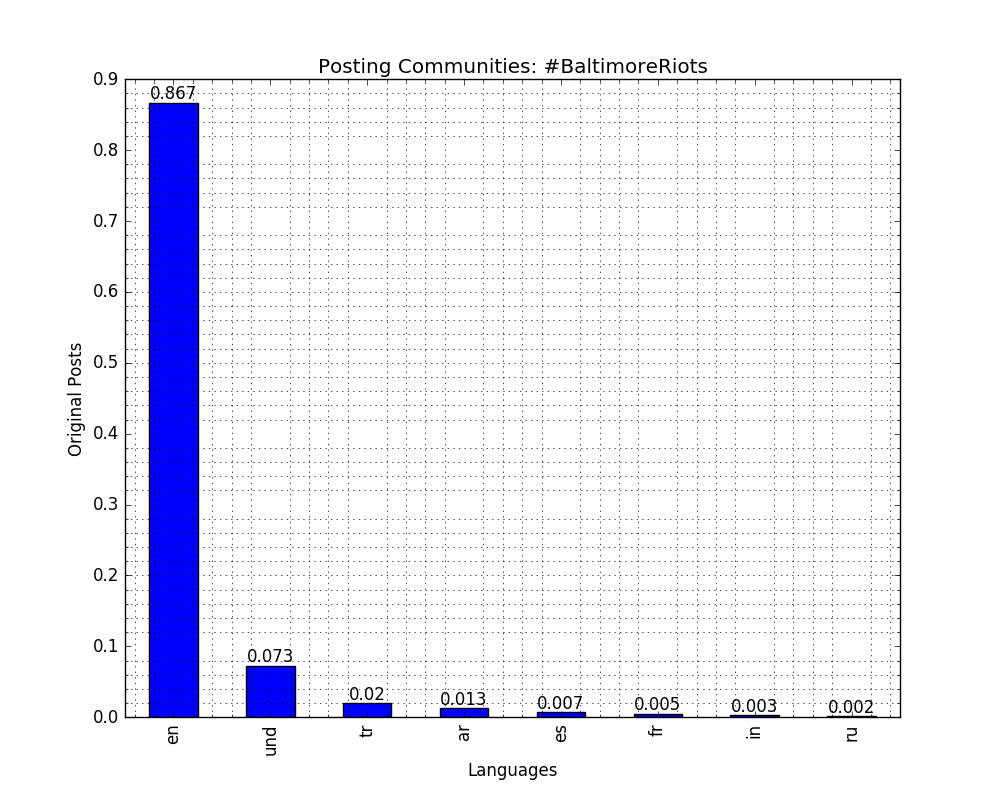
\includegraphics[width=\columnwidth]{images/baltimore_langfreq.png}
\caption{Most frequently used languages in
  {\texttt{\#BaltimoreRiots}}: 
({\emph{en:}} English; {\emph{es:}} Spanish; {\emph{tr:}} Turkish;
  {\emph{fr:}} French; {\emph{en-gb:}} British English; {\emph{ar:}}
  Arabic; {\emph{de:}} German; {\emph{ru:}} Russian; {\emph{it:}}
  Italian; {\emph{pt:}} Portuguese)}
\label{fig:baltimore_langfreq}
\end{figure}

\subsection{Users' Language Communities}

In the majority of cases, users choose to pick a language for their
Twitter profile settings. In our dataset we found that out of 716,494
users, only 45 had not chosen any language. However, the language
entity returned by the API for those cases is the initial placeholder
text ``{\emph{Select Language...}}'' or a translated version that might provide
hints regarding the user language
community. Figure~\ref{fig:baltimore_profile_size} shows that about 94\% of the
users came from `{\emph{en}}' profile community.

\begin{figure}[htb]
\centering
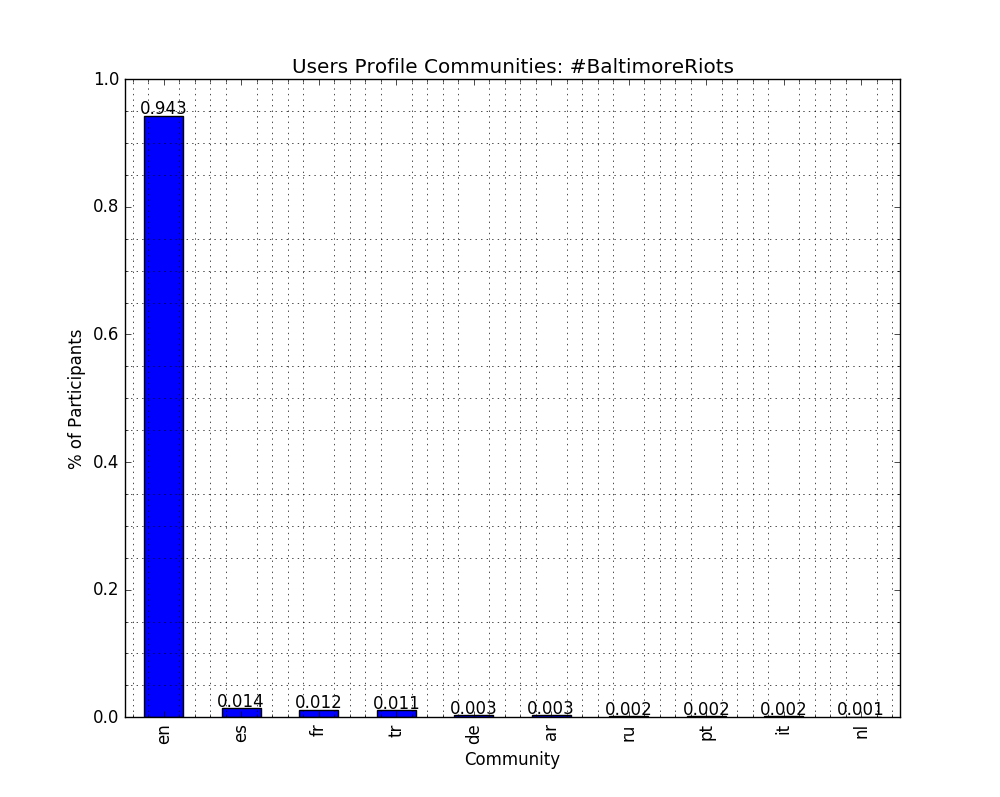
\includegraphics[width=\columnwidth]{images/baltimore_profile_size.png}
\caption{Top 10 profile language communities in {\texttt{\#BaltimoreRiots}}}
\label{fig:baltimore_profile_size}
\end{figure}

\begin{figure}[htb]
\centering
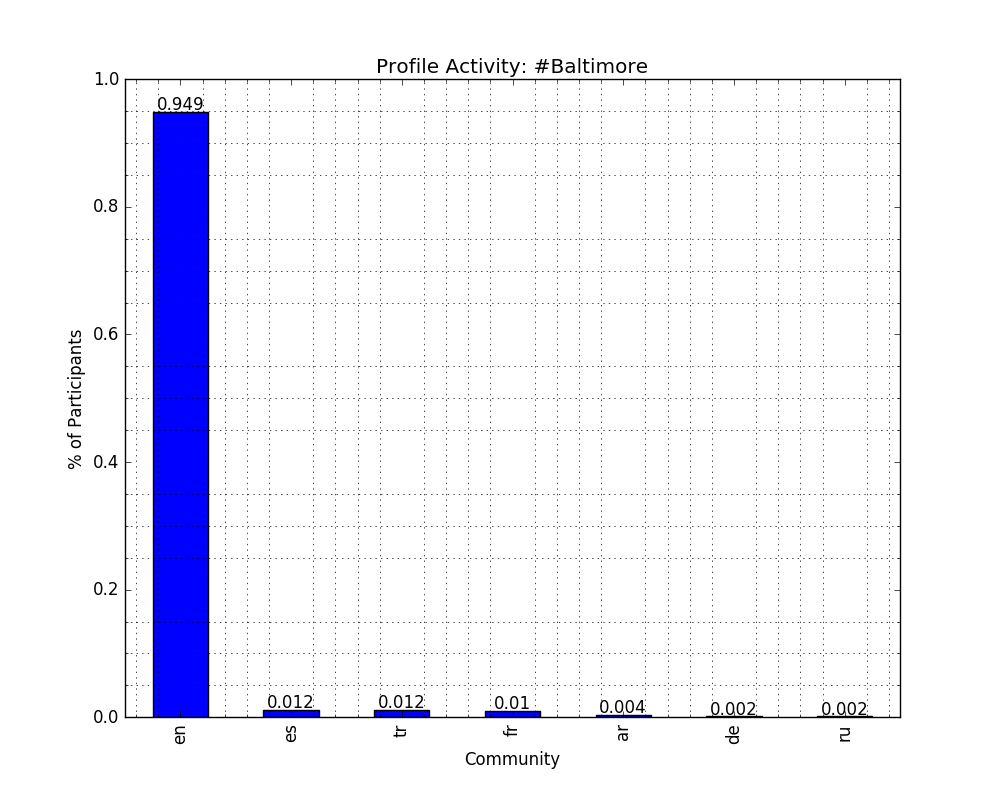
\includegraphics[width=\columnwidth]{images/baltimore_profile_activity.png}
\caption{Profile language communities casuig \%99 of activity in {\texttt{\#BaltimoreRiots}}}
\label{fig:baltimore_profile_activity}
\end{figure}

As we can see in figure ~\ref{fig:baltimore_profile_activity}, 
activity from profile communities is not far from their sizes.
Also, from these two outputs, we can see that nearly all of the topic
activity came from one particular community using one particular
language. This extreme pattern may accompany extreme and
geographically constrained real world events such as riots and terror
attacks.


\subsection{Profile-Posting Graph}
To investigate whether the `{\emph{en}}' posting community is linked to
particular profile communities, we constructed a bipartite graph as
presented in figure~\ref{fig:baltimore_p_s_lang_sl}, representing the
profile-posting language network. In this graph, nodes that are
prefixed by ``{\emph{p\_}}'' represent profile language community, and
nodes that are prefixed by ``{\emph{s\_}}'' represent posting language
community. Size of node represents the weighted indegree, whereas colour
represents the outdegree; the darker the colour, the higher
outdegree, hence, totally white nodes have no out degree and help to easly distinguish posting communities from profile ones.
The graph confirms the domination pattern we highlighted
earlier; furthermore, it shows the relationships between the profile and
posting communities. 

\begin{figure}[htb]
\centering
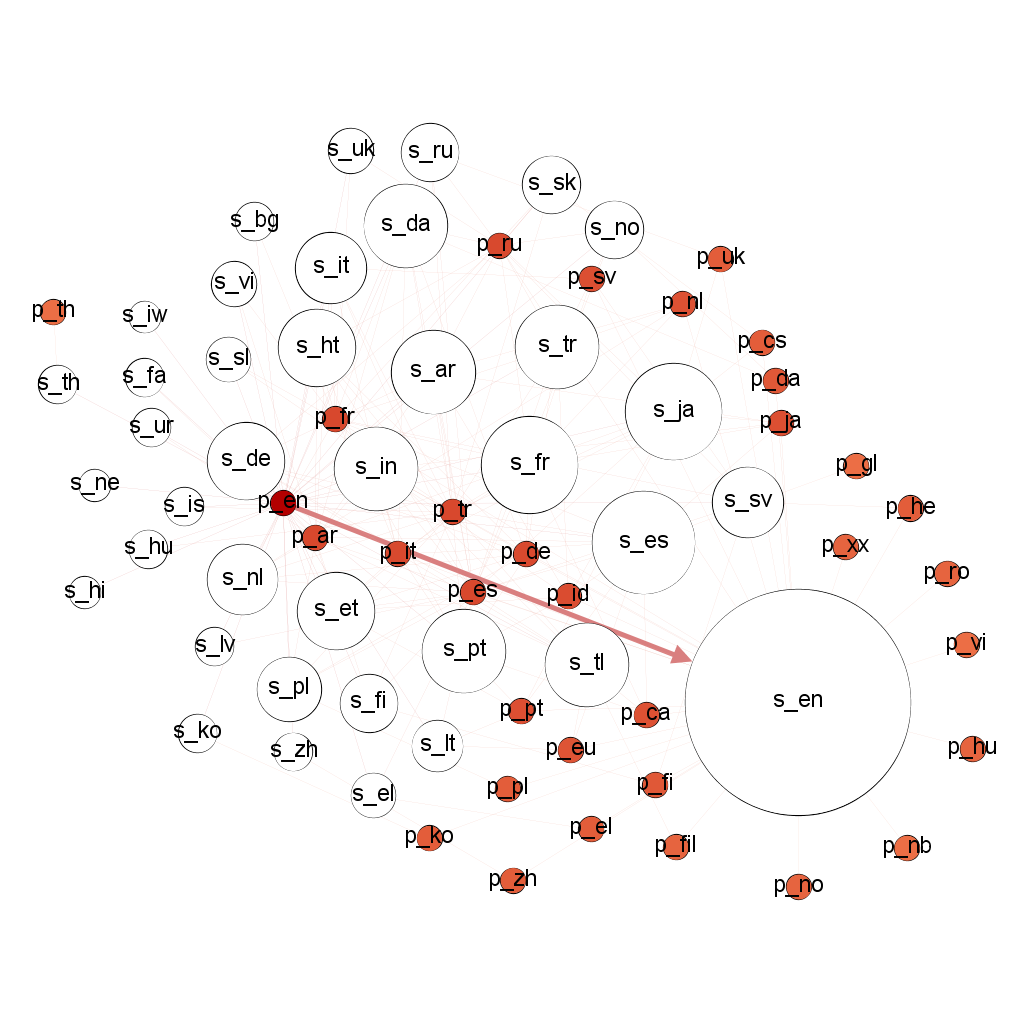
\includegraphics[width=\columnwidth]{images/baltimore_p_s_lang_sl.png}
\caption{Profile-Posting network graph, selfloop included}
\label{fig:baltimore_p_s_lang_sl}
\end{figure}

\begin{figure}[htb]
\centering
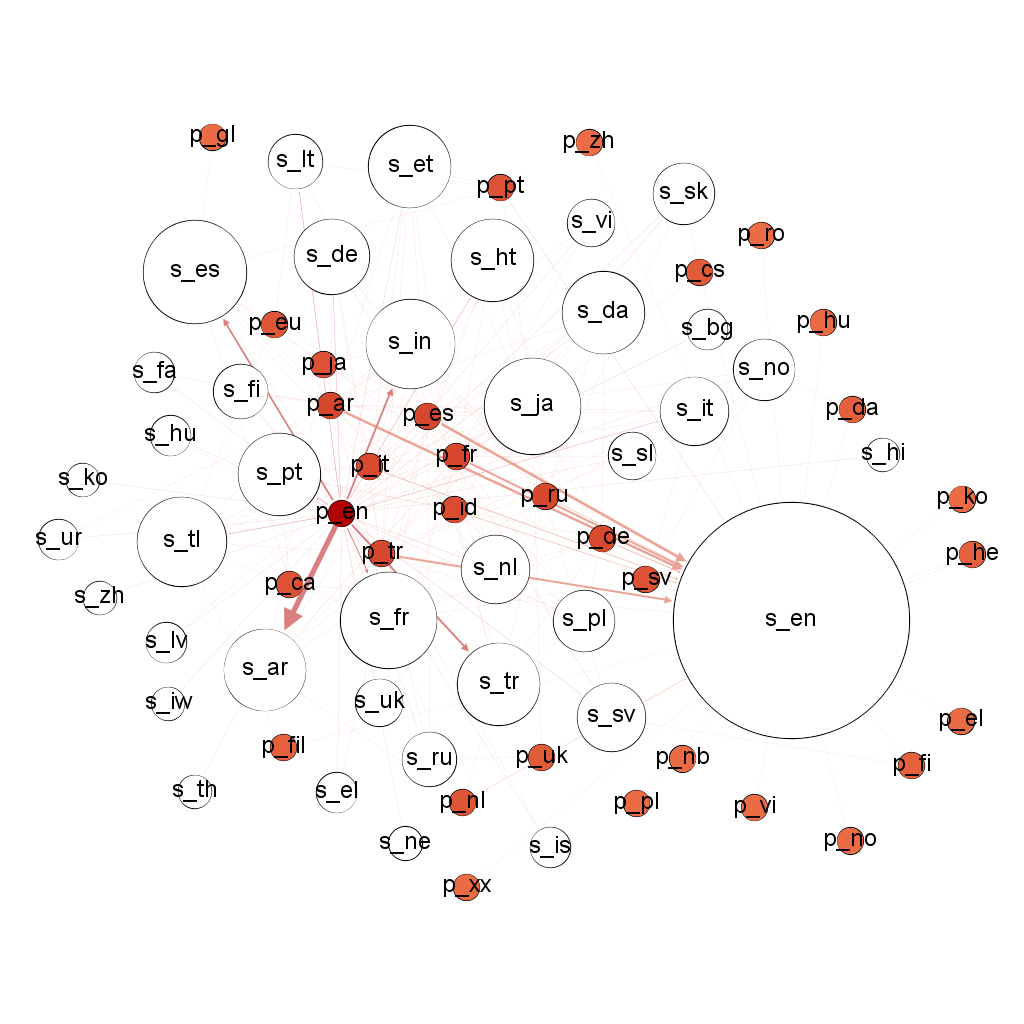
\includegraphics[width=\columnwidth]{images/baltimore_p_s_lang_nsl.png}
\caption{Profile-Posting network graph, no selfloop}
\label{fig:baltimore_p_s_lang_nsl}
\end{figure}

\begin{figure}[htb]
\centering
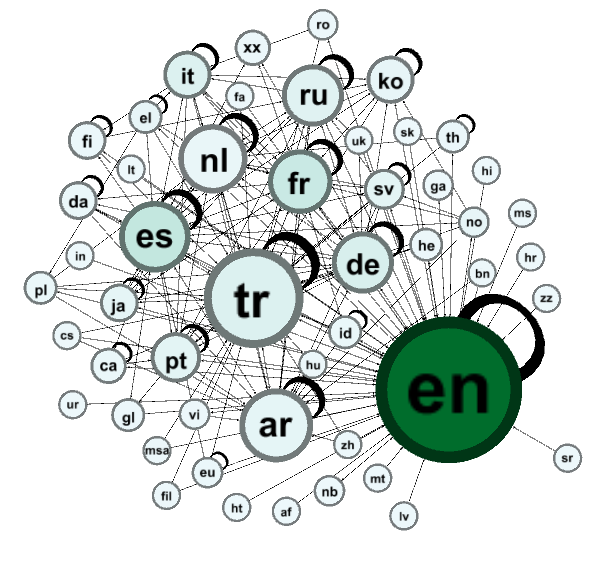
\includegraphics[width=\columnwidth]{images/baltimoreprofileprofile.png}
\caption{Profile-profile network graph}
\label{fig:baltimoreprofileprofilegraph}
\end{figure}


Furthermore, to examine users behaviour in using languages other than their own (profile language), while same-language 
communities are filtered out for clarity, the result is shown in figure ~\ref{fig:baltimore_p_s_lang_nsl}. 
In this figure, relationships can be easly observed by looking at weight of their edges. As we can see in Table~\ref{tbl:baltimoredifflang}, in this context,  
English profile users have mostly been posting in Arabic, followed by Espanish profiles posting in English. This observation shed the light on those relatioships, and could be of use for further analysis, such as highly dissiminated message that fall into these relationships and thier contents. 

\begin{table}[!htb]
\centering
\begin{tabular}{@{}lcr@{}}
\toprule
\textbf{Profile-Posting Edge} & \textbf{Weight} \\ \midrule
{\emph{en-ar}} & 1791 \\
{\emph{es-en}} & 727 \\
{\emph{ar-en}} & 697\\ 
{\emph{fr-en}} & 571 \\
{\emph{tr-en}} & 558 \\
{\emph{en-tr}} & 550 \\ \bottomrule
\end{tabular}
\caption{Users behaviour in using languages different to their profile}
\label{tbl:baltimoredifflang}
\end{table}

For an extreme case of one dominating posting language, we wanted to
investigate participation of different communities. We thus filtered
out all non-`{\emph{en}}' statuses, and then identified different
profile communities with the resultant set. For each community, we
classified statuses into two sets: {\emph{actions}} and
{\emph{reactions}}; this result is shown in
Table~\ref{tbl:mostactive}. This shows the highest scoring
communities, where the first column represents the category of status
(action or reaction), community column represents profile language
community, and last one shows percentage of `{\emph{en}}' posts by
that community.

\begin{table}[!htb]
\centering
\begin{tabular}{@{}lcr@{}}
\toprule
\textbf{Category} & \textbf{Community} & \textbf{\%} \\ \midrule
Reaction & {\emph{en}} & 81.08 \\
Action & {\emph{en}} & 15.43 \\
Reaction & {\emph{es}} & 0.68 \\
Reaction & {\emph{fr}} & 0.59 \\
Reaction & {\emph{en-gb}} & 0.47 \\
Reaction & {\emph{tr}} & 0.19 \\
Reaction & {\emph{de}} & 0.18 \\
Reaction & {\emph{pt}} & 0.13 \\ \bottomrule
\end{tabular}
\caption{Activity and categories of most active profile language
  communities}
\label{tbl:mostactive}
\end{table}

From the results above we can infer that there is a dominating player
in both domains: posting languages and profile communities. Therefore,
for the case of {\texttt{\#BaltimoreRiots}}, we can conclude that the case was
substantially localised.


\subsection{Reaction Networks}\label{reactionnetworks}

Another important perspective to identify and capture is how different
profile communities relate to each other in terms of
reactions. Therefore, we constructed the graph in
Figure~\ref{fig:baltimoreprofileprofilegraph} to show interactions amongst
language communities. Edges are directed and are drawn from reacting
nodes (retweeter, or replier) to the original acting node
(tweeter). Node size represents weighted indegree; darkness of colour indicates oudegree. The figure clearly shows that communities 
are most reactive to their own than to others.

\begin{figure}[htb]
\centering
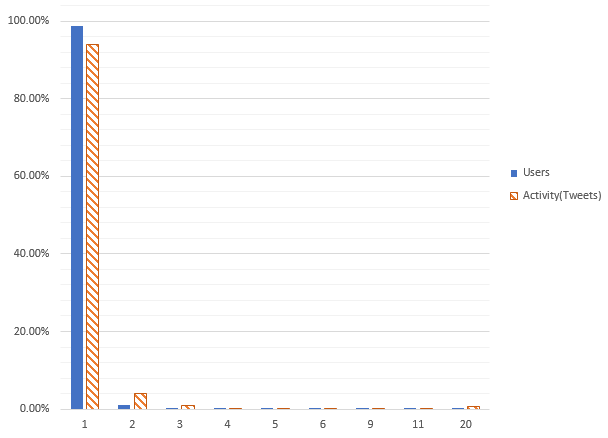
\includegraphics[width=\columnwidth]{images/baltimore_multilingual.png}
\caption{Multilingual communities and their activity in {\texttt{\#BaltimoreRiots}}}
\label{fig:baltimore_multilingual}
\end{figure}

\subsection{Multilingual Communities}
In this section, we group users based on their relationship with
posting communities, regardless of their profile language. For
example, a user posting in both `{\emph{en}}' and `{\emph{fr}}' will
be classified as bilingual, and so on. Based on this grouping
technique, with the `{\emph{und}}' lang category eliminated, we
identified 9 sets. As we can see in Figure~\ref{fig:baltimore_multilingual}, monolingual group contain most users, nearly \%99 of users, and about \%94 
of the topic activity came from this group too.

\section{Case Study: 2016 Eurovision Song
  Contest}\label{eurovisioncasestudy}

The Eurovision Song Contest ({\emph{Concours Eurovision de la
chanson}}) -- sometimes popularly called Eurovision -- is the
longest-running annual international TV song competition, held,
primarily, among the member countries of the European Broadcasting
Union since 1956. Each participating country submits an original
song to be performed on live television and radio and then casts votes
for the other countries' songs to determine the most popular song in
the competition. The contest has been broadcast every year for sixty
years, and is one of the longest-running television programmes in the
world. It is also one of the most watched non-sporting events in the
world, with audience figures varying in recent years from 100 million
to 600 million globally\footnote{\url{https://www.eurovision.tv}}. The
emergence of social networking in recent years has dramatically
changed the range and scope of audience interaction and engagement,
particularly for different language communities.

The 2016 Eurovision Song
Contest\footnote{\url{https://www.eurovision.tv/page/stockholm-2016/all-participants}}
took place in May in Stockholm, Sweden. There were 32 countries taking
part, with two semi-finals taking place on 12 and 14 May. 26 countries
qualified for the final on 16 May. This year’s contest was perceived
by many commentators to be tense and politically motivated, especially
with Ukraine eventually winning the
final~\cite{telegrapheuroboycott:2016}. Varying analyses see the
contest as being influenced by political conflicts, friendships or
cultural
bias~\cite{ginsburgh+noury:2008,charron:2013,blangiardo+baio:2014,budzinski+pannicke:2016},
with a range of news articles explicitly discussing the possibly
biased results~\cite{telegrapheurobias:2016}.  Twitter activity was
very high throughout the event on the main {\texttt{\#Eurovision}}
hashtag. The participation exceeded 7,900,000 statuses, produced by
1,226,959 users; Figure~\ref{fig:overalleurovisionactivity} shows the overall
Twitter activity.

\begin{figure}[htb]
\centering
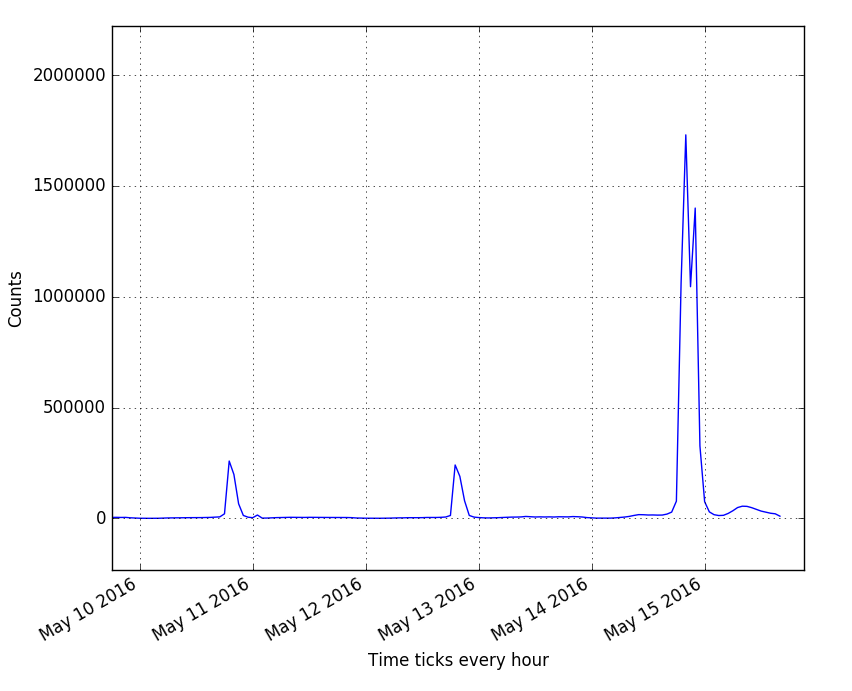
\includegraphics[width=\columnwidth]{images/overalleurovisionactivity.png}
\caption{Overall activity for {\texttt{\#Eurovision}}.}
\label{fig:overalleurovisionactivity}
\end{figure}

Preliminary analysis shows that tweets and retweets together account
for c.97\% from the total activity, as shown in
Figure~\ref{fig:overalleurovisionactivity}. These two subsets can be
representative on their own, without the need to include other
interaction sets, such as replies and quoted tweets. It is important
to note that tweets and retweets are used to measure actions, and
reactions, respectively. However, our analysis will be focusing on
original tweets only and the usage of different languages in this set.

\subsection{Locations}\label{eurovisionlocations}

As mentioned in Section~\ref{intro}, for the sake of anonymity many
users tend not to disclose information about their identity,
particularly locations; this has also been supported by the literature
that geotagged tweets are generally low in
number~\cite{kang-et-al:2013}. We took the step to verify this claim
in our datasets; in the best cases, the ratio of geotagged tweets did
not exceed 2\%. An alternative location-based option to consider is
based on profile location, but it still does not serve the need for
location clustering for a multitude of reasons. Firstly, we found that
less than 45\% of users have set their profile location, which is in
line with other studies~\cite{graham-et-al:2014}. Secondly, although
Twitter suggests certain presets for setting profile location, users
are given the option to enter any text they wish; this results in a
considerable amount of noise.

\subsection{Profile and Posting Communities}\label{ppcomm}

In the {\texttt{\#Eurovision}} case, there were 49 posting
languages. Table~\ref{tbl:activelangs} shows the top posting languages
accounted for 90\% of original posts (tweets), out of 3,834,937. As
might be expected, the English was the most used posting
language. Interestingly, the results show that the language of 142,721
(3.72\%) statuses could not be identified. When investigated further,
c.40\% of these statuses did not contain much text other than
hashtags, user mentions or URLs. Although this category shows an
interesting case in which qualitative content analysis could be
involved, it is beyond the scope of this study and will not be
addressed here.


\begin{table}[!htb]
\centering
\begin{tabular}{@{}lc}
\toprule
\textbf{Language} & \textbf{\%} \\ 
\midrule
{\emph{en}} & 45.90 \\
{\emph{es}} & 17.24 \\
{\emph{ru}} & 8.99 \\
{\emph{fr}} & 6.20 \\
{\emph{und}} & 3.72 \\
{\emph{nl}} & 3.71 \\
{\emph{de}} & 3.19 \\
{\emph{it}} & 2.85 \\ 
\bottomrule
\end{tabular}
\caption{Most active profile language
  communities, accounting for 90\% of original tweets}
\label{tbl:activelangs}
\end{table}


In total, 1,226,959 users interacted with the {\texttt{\#Eurovision}}
hashtag. In terms of their profile languages, they formed 50
communities. Table~\ref{tbl:profcomms} shows the profile communities
from the top 90\% of all users. Unlike status language, profile
language relies on the user to pick a language for their Twitter
profile settings. In general, the default value of this option is the
initial placeholder text ``{\emph{Select Language...}}'' or a
translated version that might provide hints regarding the user
language community. In our dataset, we found that all users had
selected a language and no users with the default value.


\begin{table}[!htb]
\centering
\begin{tabular}{@{}lc}
\toprule
\textbf{Community} & \textbf{\%} \\ 
\midrule
{\emph{en}} & 47.06 \\
{\emph{es}} & 20.37 \\
{\emph{fr}} & 8.00 \\
{\emph{ru}} & 7.07 \\
{\emph{de}} & 3.539 \\
{\emph{nl}} & 3.31 \\
{\emph{it}} & 2.25 \\ 
\bottomrule
\end{tabular}
\caption{Profile communities, for top 90\% of users}
\label{tbl:profcomms}
\end{table}

\subsection{Profile-Posting Analysis}

From the previous two tables, we can see some similarities between the
posting and profile communities. Taking an exceptional case as an
example, we can see that although the French profile community had
more presence, the Russian posting community is larger by 2.79\%. A
simple explanation would be that the Russian profile community was
relatively more active than French due to the focus on related
countries; another reason could be the participation of non-Russian
profiles using the Russian language for posting. To investigate this,
we investigated the contribution of profile communities to the Russian
posting community. The result in Table~\ref{tbl:russian} shows profile
communities that resulted in more than 95\% of activity in this
posting community.


\begin{table}[!htb]
\centering
\begin{tabular}{@{}lc}
\toprule
\textbf{Community} & \textbf{\%} \\ 
\midrule
{\emph{ru}} & 91.25 \\
{\emph{en}} & 7.26 \\
\bottomrule
\end{tabular}
\caption{Active profile communities within the Russian posting community}
\label{tbl:russian}
\end{table}


As we can see in this example, posts in Russian were not merely
appearing from the Russian profile community. This show one way of
exploring relationships between profile and posting communities,
especially if we are interested in particular communities.

Another approach is to explore the posting behaviour of one particular
community. When considering certain profile communities, there is a
tendency to assume that communities only post in languages that are
the same as their profile language. To examine this assumption, we
investigated participation of `{\emph{en}}' profiles, as they form
nearly 50\% of users. In total, there were 1,841,205 posts from this
community, 81\% of which were posted in `{\emph{en}}', 15.4\% in other
languages, and 3.62\% were not identified. Table~\ref{tbl:enpartlangs}
lists the top 95\% posting languages used by this profile community.


\begin{table}[!htb]
\centering
\begin{tabular}{@{}lc}
\toprule
\textbf{Language} & \textbf{\%} \\ 
\midrule
{\emph{en}} & 80.99 \\
{\emph{und}} & 3.62 \\
{\emph{es}} & 2.69 \\
{\emph{nl}} & 2.39 \\
{\emph{fr}} & 1.39 \\
{\emph{ru}} & 1.36 \\
{\emph{de}} & 0.97 \\
{\emph{it}} & 0.87 \\ 
{\emph{el}} & 0.86 \\ 
\bottomrule
\end{tabular}
\caption{Top 95\% of participation languages from `{\emph{en}}' profiles}
\label{tbl:enpartlangs}
\end{table}


\subsection{Language Diversity}

By observing the language diversity of profile communities, we aim to
measure language diversity of the topic in general, as well as
investigating which community plays a key role in bridging different
profile communities. Diversity in this context means how many posting
languages were used from each profile community, and to what extent
they used their own language, as well as other languages.  The general
language diversity of the topic is c.17\%, while 3.72\% were not
identified. All of the 50 profile communities used different languages
in posting. Interestingly, 16 out of those communities did not use
their own language, they were low in participation though. Moreover,
in terms of using different languages, we found that 32 communities
scored at least 50\% out of their tweets. We noticed that posting from
small profile communities may affect the overall language diversity of
the topic. Referring to the top profile communities discussed in
Section~\ref{ppcomm}, Table~\ref{tbl:diversity} shows their
diversity by percentage. The Russian profile community is again an
interesting case, as it scored the least diverse profile amongst all
the 50 communities although it comes fourth in number of users.


\begin{table}[!htb]
\centering
\begin{tabular}{@{}lc}
\toprule
\textbf{Language} & \textbf{\%} \\ 
\midrule
{\emph{de}} & 34.27 \\
{\emph{nl}} & 32.78 \\
{\emph{it}} & 18.49 \\ 
{\emph{fr}} & 16.65 \\
{\emph{en}} & 15.39 \\
{\emph{es}} & 10.13 \\
{\emph{ru}} & 7.93 \\
\bottomrule
\end{tabular}
\caption{Diversity of the top profile communities}
\label{tbl:diversity}
\end{table}


\subsection{Multilingual Communities}

In this section, we group users based on their relationship with
posting communities, regardless of their profile language. For
example, a user posting in both `{\emph{en}}' and `{\emph{fr}}' will
be classified as bilingual, and so on. Based on this grouping
technique, with the `{\emph{und}}' lang category eliminated, we
identified 20 sets. The smallest two groups consist of one user each,
who posted in 22 and 25 different languages.  As we can see in
Figure~\ref{fig:multilingual}, monolingual users scored about 85\% of
all users, creating 47\% of the total original posts. The also shows
that users and their activity decrease as number of languages used
increase.


\begin{figure}[htb]
\centering
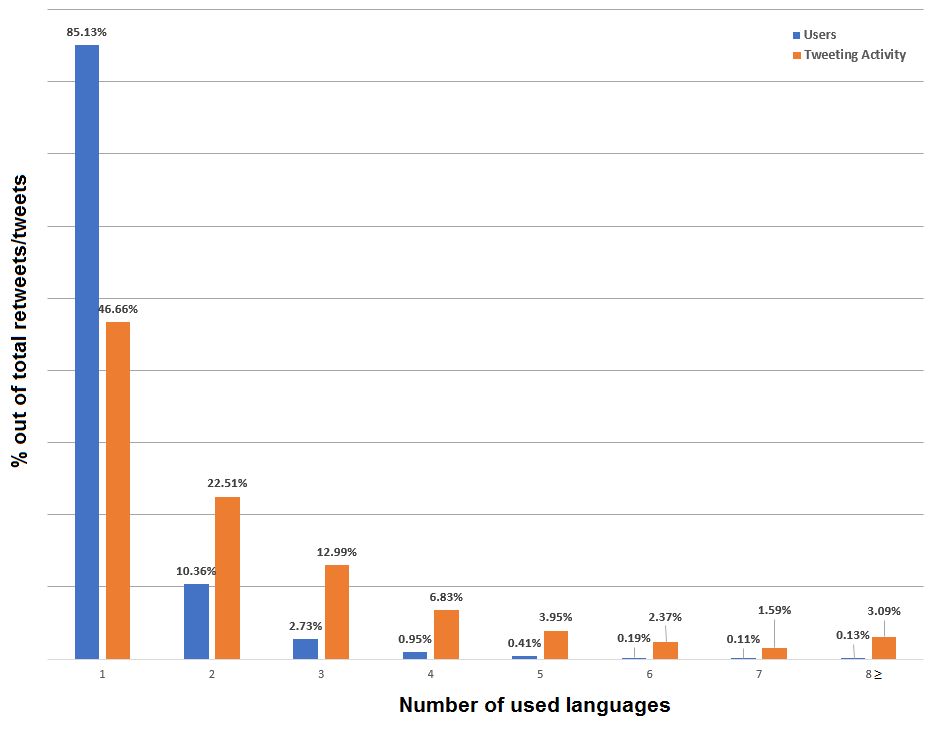
\includegraphics[width=\columnwidth]{images/multilingualcommunities.png}
\caption{Multilingual communities and their associated activities.}
\label{fig:multilingual}
\end{figure}


A closer look at the behavior of these communities shows that, in
general, activity per user increases as number of used languages
increase, as shown in
Figure~\ref{fig:multilingualpostsperuser}. Although we cannot conclude
that there is a correlation between high multilingualism and
illegitimacy of accounts, this would be an interesting further topic
to investigate.


\begin{figure}[htb]
\centering
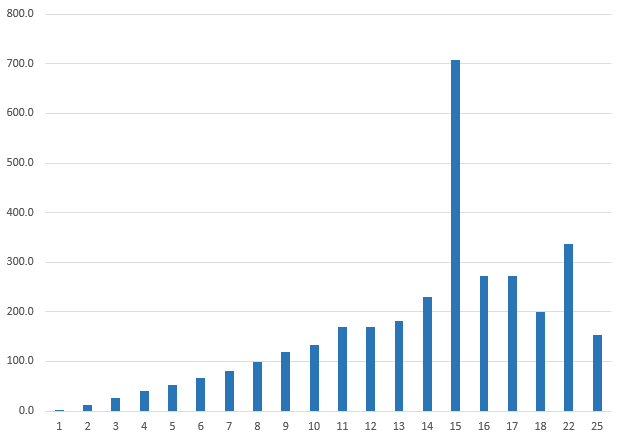
\includegraphics[width=\columnwidth]{images/multilingualpostsperuser.png}
\caption{Average number of posts per user for multilingual communities.}
\label{fig:multilingualpostsperuser}
\end{figure}


\section{Conclusions}\label{conclusions}

This paper presents two real-world case studies -- the 2015 Baltimore
protests in the USA and the 2016 Eurovision Song Contest -- in
identifying languages used, language and multilingual communities, and
their engagement and interactions on the Twitter platform. As we
discussed in Section~\ref{langcomm}, the nature of the event
(e.g. being a local or global) may be reflected on community
conversations on Twitter. We found that most of posting activity comes
from the main community (the language community in which the incident
has happened or tightly related to). This is especially the case when
the online conversations are triggered by a real world incident. The
same for posting languages, users mostly to use the language of the
main community. Although most of topic activity comes from that main
community, we noticed that, with local events, other communities work,
mostly, as information spreaders. Furthermore, there is a positive
relationship between size of profile and posting communities; we have
also showed that a large number in participating profile community
does not necessarily imply high language diversity, and that diversity
may results from small profile community. We also presented the
structure of multilingual communities and their activity. Although
most users may use their own profile language in posting, most of the
activity came from multilingual users. In a few cases, users may use a
significant number of languages, up to 25 different languages. These
extreme cases may be interesting to investigate for possible
spammer/false account detection or for sociolinguistics in more
moderate cases.

We also presented a network graph (using
Gephi\footnote{\url{https://gephi.org/}} and the Networkx Python
package\footnote{\url{https://networkx.github.io/}}) showing how
language communities relate to each other in the form of
action-reaction (action: tweet, reaction: retweet, reply,
quote). Another interesting graph that we produced to show relations
between profile and posting communities. We find that this graph is
important to facilitate comparing users defined profile language with
their posting language. Some event might be termed as `partially
scheduled' as their end was different to how they were planned in the
first place. In such tense situation, we noticed that diversity of
languages and communities are very low, and there always be a
dominating community and language.

The method we presented here can be used in identifying how
communities interact with one another, which ones are most active,
which languages are mostly used, and at what time. Applying these
techniques on data pouring from the Twitter Stream
API\footnote{\url{https://dev.twitter.com/streaming/overview}} would
be applicable to a wide number of domains. For example, these methods
can be used in social network marketing and publicity to increase the
probability of influential posts. In practice, for a given
{\texttt{\#<Brand>}}, by monitoring the activity of different language
community, one can decide the time to post well-tailored tweets
targeting certain communities. This can be fine-tuned further by
mentioning key players in that community, e.g. users with high
closeness scores.

Moreover, within certain contexts, the order of applying these two
classifications (posting and profile) will generate different results.
For example, taking one profile community and dividing it into
different posting communities shows the number of languages this
community may use, and hence degree of openness and reachability. A
possible scenario for governments, politicians or campaigners would be
to use this method to measure to what extent other languages are used
within a profile community. It may also show how users associate
themselves with one community in their profile while using other
languages. Monitoring unusual activity for secondary languages may
help to uncover important messages or opinions that could not be
openly expressed, for a variety of reasons, to the rest of the profile
community. For the social network analysis domain, this method
provides a different perspective for influence analysis. Endorsement
from different profile communities cannot be measured similar to those
coming from the same community. For example, in a controversial Arabic
topic, we noticed that high support came from other profile
communities.

The method we presented here can be used in identifying how
communities interact with one another, which ones are most active,
which languages are mostly used, and at what time. Moreover, within
certain contexts, the order of applying these two classifications
(posting and profile) will generate results in different
perspectives. For example, taking one profile community and dividing
it into different posting communities shows the number of languages
this community may use, and hence degree of openness and
reachability. A possible scenario for governments, politicians or
campaigners would be to use this method to measure to what extent
other languages are used within a profile community. It may also show
how users associate themselves with one community in their profile
while using other languages. Monitoring unusual activity for secondary
languages, in multilingual communities, may help to uncover important
messages or opinions that could not be openly expressed, for a variety
of reasons, to the rest of the profile community.

For future work, we plan to have a deeper look at how multilingual
communities participate and their reaction networks. We believe that
differentiation between endorsements (e.g. retweets) and other
reactions may provide further insight into the networks and
communities. Also, we plan to add further classifications to the
reaction network (as presented in Section~\ref{reactionnetworks}). We
believe that differentiation between endorsements (e.g. retweets) and
other reactions may provide further insight into the networks and
communities. Furthermore, we will apply the methods presented in this
paper on other high-profile event/discussion datasets in different
domains or contexts, such as for sports, music contests and civil
rights/humanitarian actions.



% \subsection{References}
% Generated by bibtex from your \texttt{.bib} file.  Run latex,
% then bibtex, then latex twice (to resolve references)
% to create the \texttt{.bbl} file.  Insert that \texttt{.bbl}
% file into the \texttt{.tex} source file and comment out
% the command \texttt{{\char'134}thebibliography}.


\begin{acks}
This work has been supported by a doctoral research scholarship for
Nabeel Albishry from King Abdulaziz University, Kingdom of Saudi
Arabia.
\end{acks}
